\documentclass[tikz]{standalone}
% To convert from pdf to png use the following :
%
% C:\cygwin64\bin\convert.exe -density 600 switch.pdf -resize 240x240 switch.png
%

\usepackage{listings}

\usetikzlibrary{positioning}
\usetikzlibrary{calc}
\usetikzlibrary{backgrounds}
\usetikzlibrary{decorations.text}

\begin{document}
%
% Importer : Encased
%
% This traps the import at multiple entry points representing 
% the most complete importer one may produce.
%

% Anti-spokes
%
% The idea is to draw an anti-spoke or paddles with this diagram.
%
% \begin{tikzpicture}
% \draw let \n{spokes}={3}, \n{arc}={360/\n{spokes}}, \n{angoff}={-\n{arc}+30} in foreach[evaluate = \idx as \ray using \idx/\n{spokes}*360] \idx in {1,2,...,\n{spokes}}
%  {(0,0) -- (\ray+\n{angoff}:1em) (\ray+\n{angoff}+\n{arc}/2:2em) -- (\ray+\n{angoff}-\n{arc}/2:2em)};
% \end{tikzpicture}
%
%
% \begin{tikzpicture}
% \draw [rounded corners]
%   let \n{spokes}={3}, 
%       \n{arc}={360/\n{spokes}}, \n{angoff}={-\n{arc}+30}, 
%       \n{Radius}={6em}, \n{radius}={1em} 
%   in foreach[evaluate = \idx as \ray using \idx/\n{spokes}*360] \idx in {1,2,...,\n{spokes}}
%  {(\ray+\n{angoff}:\n{radius}) -- (\ray+\n{angoff}+\n{arc}/2:\n{Radius}) -- (\ray+\n{angoff}-\n{arc}/2:\n{Radius}) -- cycle};
% \end{tikzpicture}

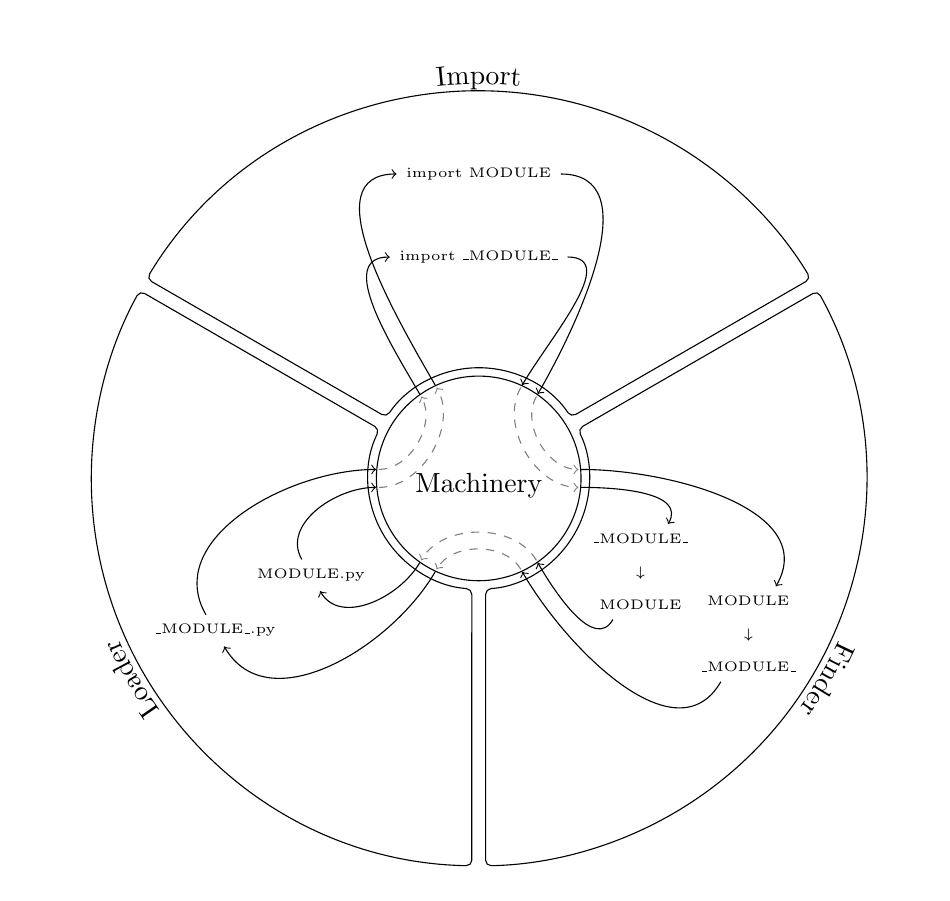
\begin{tikzpicture}[
 arc label/.style={
  decorate,
  decoration={ 
   text along path,
   text align=center,
   reverse path=true,
   text={#1}
   }}]
\coordinate (ctr) {}; % Used as an anchor for later nodes
% Import Mechanism
%
% Originally this was drawn using a series of sectors
%
% \fill[gray, opacity=50, rounded corners=1em] ($(ctr) + (10:1em)$) -- ($(ctr) + ( 30:15em)$) arc( 30:150:15em) -- cycle;
% \fill[gray, opacity=50, rounded corners=1em] ($(ctr) + (10:1em)$) -- ($(ctr) + (150:15em)$) arc(150:270:15em) -- cycle;
% \fill[gray, opacity=50, rounded corners=1em] ($(ctr) + (10:1em)$) -- ($(ctr) + ( 30:15em)$) arc( 30:-90:15em) -- cycle;
%
% This was superceeded by a sector drawing command that formally accounted for spokes.
%
% \draw [rounded corners]
%   let
%    \n{spokes}={3}, 
%    \n{radius}={1em}, \n{Radius}={6em},
%    \n{width}={0.25em},
%    \n{arc}={360/\n{spokes}},
%    \n{innerarc}={\n{arc}/2-2*asin(\n{width}/2/\n{radius})}, \n{outerarc}={\n{arc}/2-2*asin(\n{width}/2/\n{Radius})},
%    \n{angoff}={\n{arc}/2+30}
%   in foreach [evaluate = \idx as \ray using \idx/\n{spokes}*360] \idx in {1,2,...,\n{spokes}}
%  {(\ray+\n{angoff}+\n{innerarc}:\n{radius}) arc(\ray+\n{angoff}+\n{innerarc}:\ray+\n{angoff}-\n{innerarc}:\n{radius}) -- 
%   (\ray+\n{angoff}-\n{outerarc}:\n{Radius}) arc(\ray+\n{angoff}-\n{outerarc}:\ray+\n{angoff}+\n{outerarc}:\n{Radius}) -- cycle};
%
% This was again superceeded by a varsion that accounted for labels
%
\foreach 
  [var=\spokes,  evaluate=\spokes using    3,
   var=\radius,  evaluate=\radius using    4, 
   var=\Radius,  evaluate=\Radius using    14, 
   var=\width,   evaluate=\width  using 0.25, 
   var=\offset,  evaluate=\offset using 0.25, 
   var=\arc,     evaluate=\arc    using 360/\spokes,
   var=\inner,   evaluate=\inner  using {\arc/2-2*asin(\width/2/\radius)},
   var=\outer,   evaluate=\outer  using {\arc/2-2*asin(\width/2/\Radius)},
   var=\rotate,  evaluate=\rotate using \arc/2+30,
   count=\count from 0, evaluate = \idx as \ray using \count/\spokes*360] \text in {Import, Loader, Finder} 
  {\draw [rounded corners = 0.2em]
     (\ray+\rotate-\inner:\radius em) arc(\ray+\rotate-\inner:\ray+\rotate+\inner:\radius em) -- 
     (\ray+\rotate+\outer:\Radius em) arc(\ray+\rotate+\outer:\ray+\rotate-\outer:\Radius em) -- cycle;
   \draw[arc label = \text] let \n{radius} = {\offset+\Radius} in (\rotate+\ray-\outer:\n{radius} em) arc (\rotate+\ray-\outer:\rotate+\ray+\outer:\n{radius} em);};
% \node (int) at (ctr)                 [draw, fill=black, text=white, circle, inner sep = 1em] {Machinery};
% Overlay Mechanism
\node[align=center] (imp) at ($(ctr) + ( 90:    8em)$) {\lstinline[basicstyle=\tiny]|import _MODULE_|};
\node[align=center] (fdr) at ($(ctr) + (-30: 6.75em)$) {\lstinline[basicstyle=\tiny]|_MODULE_| \\ \tiny{$\downarrow$} \\ \lstinline[basicstyle=\tiny]|MODULE|};
\node[align=center] (ldr) at ($(ctr) + (210:    7em)$) {\lstinline[basicstyle=\tiny]|MODULE.py|};
\node[align=center] (Imp) at ($(ctr) + ( 90:   11em)$) {\lstinline[basicstyle=\tiny]|import MODULE|};
\node[align=center] (Fdr) at ($(ctr) + (-30:11.25em)$) {\lstinline[basicstyle=\tiny]|MODULE| \\ \tiny{$\downarrow$} \\ \lstinline[basicstyle=\tiny]|_MODULE_|};
\node[align=center] (Ldr) at ($(ctr) + (210:   11em)$) {\lstinline[basicstyle=\tiny]|_MODULE_.py|};
\node (int) at (ctr)                 [draw, circle, inner sep = 1em, align=center] {\\ Machinery};
% % Internal Structure
\draw[->, shorten >=0.1em, shorten <=0.1em, gray, dashed]  (int.65) to [out = 240, in = 180] (int.355);
\draw[->, shorten >=0.1em, shorten <=0.1em, gray, dashed] (int.185) to [out =   0, in = -60] (int.115);
\draw[->, shorten >=0.1em, shorten <=0.1em, gray, dashed] (int.305) to [out = 120, in =  60] (int.235);
\draw[->, shorten >=0.1em, shorten <=0.1em, gray, dashed]  (int.55) to [out = 240, in = 180]   (int.5);
\draw[->, shorten >=0.1em, shorten <=0.1em, gray, dashed] (int.175) to [out =   0, in = -60] (int.125);
\draw[->, shorten >=0.1em, shorten <=0.1em, gray, dashed] (int.295) to [out = 120, in =  60] (int.245);
% Primary Import
\draw[->]   (int.5) to [in =  60, out =   0]     (Fdr);
\draw[->]     (Fdr) to [in = 300, out = 240] (int.295);
\draw[->] (int.125) to [in = 180, out = 120]     (imp);
\draw[->]     (Imp) to [in =  60, out =   0]  (int.55);
\draw[->] (int.245) to [in = 300, out = 240]     (Ldr);
\draw[->]     (Ldr) to [in = 180, out = 120] (int.175);
% Secondary Import
\draw[->] (int.355) to [in =  60, out =   0]     (fdr);
\draw[->]     (fdr) to [in = 300, out = 240] (int.305);
\draw[->] (int.115) to [in = 180, out = 120]     (Imp);
\draw[->]     (imp) to [in =  60, out =   0]  (int.65);
\draw[->] (int.235) to [in = 300, out = 240]     (ldr);
\draw[->]     (ldr) to [in = 180, out = 120] (int.185);
% Swooping Structure
% \draw (imp) to[out =   0, in =  60] (fdr);
% \draw (fdr) to[out = 240, in = 300] (ldr);
% \draw (ldr) to[out = 120, in = 180] (Imp);
% \draw (Imp) to[out =   0, in =  60] (Fdr);
% \draw (Fdr) to[out = 240, in = 300] (Ldr);
% \draw (Ldr) to[out = 120, in = 180] (imp);
\end{tikzpicture}

\end{document}